\documentclass[10pt]{beamer}

\usepackage[utf8]{inputenc}
\usepackage{tcolorbox}
\usepackage{tikz}
\usepackage{tikz-3dplot}
\usetikzlibrary{intersections,calc,,angles,quotes,through}
\usepackage{amsmath}
\usepackage{graphicx}
\usepackage{cases}
\def \heart {\textcolor{blue}{$\heartsuit$} }
\def \C {\mathcal{C}}
\def \orthog {\underline{\perp}}
\def\arcos{\operatorname{arcos}}
\def \deg {^{\circ}}

\newcommand{\vect}[1] {
  \overrightarrow{#1}}

\tcbset{%
	basic/.style={colframe=black,
		      colback=white,
		      top= 0mm,
		      bottom = 2mm,
		      boxsep=0mm
		      }
}
\tikzset{
    invisible/.style={opacity=0},
    visible on/.style={alt={#1{}{invisible}}},
    alt/.code args={<#1>#2#3}{%
      \alt<#1>{\pgfkeysalso{#2}}{\pgfkeysalso{#3}} % \pgfkeysalso doesn't change the path
    },
  }

    
\begin{document}  
    \beamertemplatenavigationsymbolsempty
    \setlength{\abovedisplayskip}{0pt}
    \setlength{\belowdisplayskip}{0pt}
    \frame{
	  
	  \frametitle{Produit scalaire.}
	  \begin{figure}[h]
				  \begin{tikzpicture}[scale=0.85]
			          %projection ($(X)!(B')!(B)$)
			          %nommer chemin 'name path
			          %intersection \path [name intersections={of=d and gb,by=G}];
			          
			          %\draw[help lines] (-3,-3) grid (3,3);
			          \coordinate[label=below:$A$](A) at (0,0);
			          \coordinate[label=above:$B$](B) at (2,2);
			          \coordinate[label=below:$C$](C) at (4,0);
			          \coordinate[label=below:$B_{\bot}$](B_bot) at (2,0);
			          \draw[->] (A) -- (B);
			          \draw[->] (A) -- (C);
			          \draw[dotted] (B) -- (B_bot);
			          \pic [draw,"$\alpha$", angle eccentricity=1.5] {angle = C--A--B};
			         % \pic [draw, angle eccentricity=1.5] {angle = A--B--D};
				  \end{tikzpicture}
				  \end{figure}
				  Produit scalaire est un opération qui associe à 2 vecteurs un nombre. \\
				  \begin{align*}
				  \vect{AB}\cdot\vect{AC}=&\ |AC||AB|\operatorname{cos}(\alpha), \\[0.5em]
							 =&\ |AC||AB_{\bot}|. 
				  \end{align*}
				  
    }

    \frame{ \frametitle{Produit vectoriel.}
				  \begin{figure}[h]
				  \begin{tikzpicture}[scale=0.85]
			          %projection ($(X)!(B')!(B)$)
			          %nommer chemin 'name path
			          %intersection \path [name intersections={of=d and gb,by=G}];
			          
			          %\draw[help lines] (-3,-3) grid (3,3);
			          \coordinate[label=above right:$A$](A) at (0,0,0);
			          \coordinate[label=above:$B$](B) at (2,0,0);
			          \coordinate[label=below:$C$](C) at (0,0,1.5);
			          \coordinate[label=above:$D$](D) at (0,3,0);
			          \draw[->] (A) -- (B);
			          \draw[->] (A) -- (C);
			          \draw[->] (A) -- (D);
			          \draw[dotted] (-0.5,0,3) -- (3,0,3) -- (3,0,-1.5) -- (-0.5,0,-1.5) -- cycle;
			          \pic [draw,"$\alpha$", angle eccentricity=1.5,angle radius = 3mm] {angle = C--A--B};
			         % \pic [draw, angle eccentricity=1.5] {angle = A--B--D};
				  \end{tikzpicture}
				  \end{figure}
				  Produit vectoriel est une opération qui associe à 2 vecteurs un autre vecteur. Il est perpendiculaire aux 2 premiers.
				  Sa longueur vaut \\
				  $$|\vect{AB}\wedge\vect{AC}|\ =\ |\vect{AD}|\ =\ |AB||AC|\operatorname{sin}(\alpha).$$
    }
    \frame{ \frametitle{Centre de gravité.}\centering
    $O$, un point quelconque. 
    \begin{columns}[b]
     \column{.5\textwidth}\centering
				  \begin{figure}[h]
				  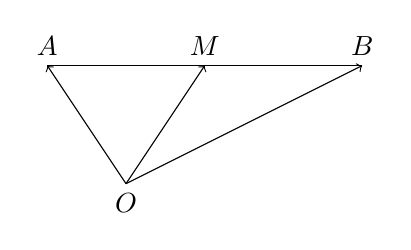
\begin{tikzpicture}[scale=1]
			          %projection ($(X)!(B')!(B)$)
			          %nommer chemin 'name path
			          %intersection \path [name intersections={of=d and gb,by=G}];
			          
			          %\draw[help lines] (-3,-3) grid (3,3);
			          \coordinate[label=above:$A$](A) at (0,0);
			          \coordinate[label=above:$B$](B) at (4,0);
			          \coordinate[label=above:$M$](M) at (2,0);
			          \coordinate[label=below:$O$](O) at (1,-1.5);
			          \draw (A) -- (B);
			          \draw[->] (O) -- (A);
			          \draw[->] (O) -- (B);
			          \draw[->] (O) -- (M); 
			         % \pic [draw, angle eccentricity=1.5] {angle = A--B--D};
				  \end{tikzpicture}
				  \end{figure}
				  $M$ milieu de $[AB]$. \\ \bigskip 
				  $\vect{OM}=\dfrac{1}{2}\vect{OA}+\dfrac{1}{2}\vect{OB}$.
     \column{.5\textwidth}\centering
				  \begin{figure}[h]
				  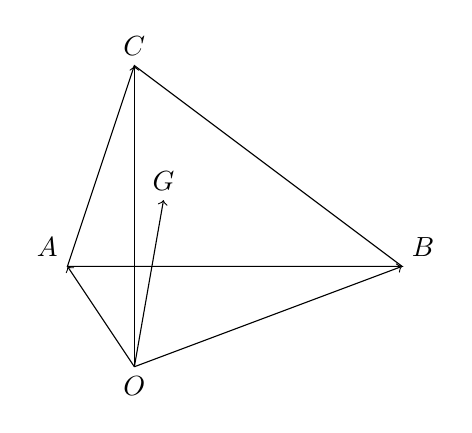
\begin{tikzpicture}[scale=0.85]
			          %projection ($(X)!(B')!(B)$)
			          %nommer chemin 'name path
			          %intersection \path [name intersections={of=d and gb,by=G}];
			          
			          %\draw[help lines] (-3,-3) grid (3,3);
			          \coordinate[label=above left:$A$](A) at (0,0);
			          \coordinate[label=above right:$B$](B) at (5,0);
			          \coordinate[label=above:$C$](C) at (1,3);
			          \coordinate[label=above:$G$](G) at ($(A)!.33!(B)!.33!(C)$);
			          \coordinate[label=below:$O$](O) at (1,-1.5);
			          \draw (A) -- (B) -- (C) -- cycle;
			          \draw[->] (O) -- (A);
			          \draw[->] (O) -- (B);
			          \draw[->] (O) -- (C);
			          \draw[->] (O) -- (G); 
			         % \pic [draw, angle eccentricity=1.5] {angle = A--B--D};
				  \end{tikzpicture}
				  \end{figure}
				  $G$ centre de gravité de $\Delta ABC$. \\ \bigskip
				  $\vect{OG}=\dfrac{1}{3}\vect{OA}+\dfrac{1}{3}\vect{OB}+\dfrac{1}{3}\vect{OC}$.
				  
    \end{columns}

    }
  
\end{document}
